% This is text associated with the open textbook "Open Electromagnetics"
% See immediately below for author, date
% This work is licensed under the Creative Commons Attribution-ShareAlike 4.0 International License. (CC BY-SA 4.0) 
% To view a copy of the license, visit http://creativecommons.org/licenses/by-sa/4.0/

%ORB TITLE Quarter-Wavelength Transmission Line
%ORB AUTHOR 0        # S.W. Ellingson, Virginia Tech (ellingson@vt.edu)
%ORB DATE 20180802   # yyyymmdd
%ORB ABSTRACT Quarter-Wavelength Transmission Line

\label{m0091_Quarter-Wavelength_Transmission_Line} % <-- Must match name of this file and module directory name.  Don't mess with this!
\index{transmission line!quarter-wavelength|(}

Quarter-wavelength sections of transmission line play an important role in many systems at radio and optical frequencies. 
The remarkable properties of open- and short-circuited quarter-wave line are presented in Section~\ref{m0088_Input_Impedance_for_Open_and_Short_Circuit_Terminations} and should be reviewed before reading further.
In this section, we perform a more general analysis, considering not just open- and short-circuit terminations but any terminating impedance, and then we address some applications.

The general expression for the input impedance of a lossless transmission line is (Section~\ref{m0087_Input_Impedance_of_a_Terminated_Lossless_Transmission_Line}):
%
\begin{equation}
Z_{in}(l) = Z_0 \frac{ 1 + \Gamma e^{-j2\beta l} }{  1 - \Gamma e^{-j2\beta l} }
\label{m0093_eZ}
\end{equation}
%
Note that when $l=\lambda/4$:
%
\begin{equation}
2\beta l = 2 \cdot \frac{2\pi}{\lambda} \cdot \frac{\lambda}{4} = \pi 
\nonumber
\end{equation}
%
Subsequently:
%
\begin{equation}
\begin{split}
Z_{in}(\lambda/4) &= Z_0 \frac{ 1 + \Gamma e^{-j\pi} }{  1 - \Gamma e^{-j\pi} } \\
                  &= Z_0 \frac{ 1 - \Gamma }{  1 + \Gamma }
\end{split}
\end{equation}
%
Recall that (Section~\ref{m0087_Input_Impedance_of_a_Terminated_Lossless_Transmission_Line}):
%
\begin{equation}
\Gamma = \frac{Z_L-Z_0}{Z_L+Z_0}
\end{equation}
%
Substituting this expression and then multiplying numerator and denominator by $Z_L+Z_0$, one obtains
%
\begin{equation}
\begin{split}
Z_{in}(\lambda/4) &= Z_0 \frac{ \left( Z_L + Z_0\right) - \left(Z_L - Z_0\right) }{ \left( Z_L + Z_0\right) + \left(Z_L - Z_0\right)  } \\
                  &= Z_0 \frac{ 2Z_0 }{  2Z_L }
\end{split}
\end{equation}
%
Thus,
%
\begin{equation}
\boxed{
Z_{in}(\lambda/4) = \frac{Z_0^2 }{  Z_L }
}
\label{m0091_eQWII}
\end{equation}
%
Note that the input impedance is inversely proportional to the load impedance.
For this reason, a transmission line of length $\lambda/4$ is sometimes referred to as a \emph{quarter-wave inverter} 
\index{quarter-wave inverter}
or simply as a \emph{impedance inverter}.
\index{impedance inverter}

Quarter-wave lines play a very important role in RF engineering.
As impedance inverters, they have the useful attribute of transforming small impedances into large impedances, and vice-versa -- we'll come back to this idea later in this section.
First, let's consider how quarter-wave lines are used for impedance matching.  
Look what happens when we solve Equation~\ref{m0091_eQWII} for $Z_0$:
%
\begin{equation}
Z_0 = \sqrt{Z_{in}(\lambda/4) \cdot Z_L }
\label{m0091_eQWZ0}
\end{equation}
%
This equation indicates that we may match the load $Z_L$ to a source impedance (represented by $Z_{in}(\lambda/4)$) simply by making the characteristic impedance equal to the value given by the above expression and setting the length to $\lambda/4$.
The scheme is shown in Figure~\ref{m0091_fQWM}.
%
\begin{figure}
\begin{center}
\pdftooltip{{  % note double braces
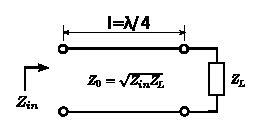
\includegraphics[width=2.5in]{modules/m0091_fQWM.eps}
}}{A transmission line with two nodes on both the input and output branches. Starting at the top left and going clockwise, l equals lambda divided by 4 and is measured between the source terminal and the load terminal.}
\end{center} 
\caption{\label{m0091_fQWM}Impedance-matching using a quarter-wavelength transmission line.}
\end{figure}

%%%%%%%%%%%%%%%%%%%%%%%%%%%%%%%%%%%%%%%%%%%%%%%%%%%%%%%%%%%%%%%

%ORB EXAMPLE
~\\ \begin{example} 
\begin{mdframed}[backgroundcolor=brown!20,linecolor=brown!20]\raggedright
300-to-$50~\Omega$ match using an quarter-wave section of line. 
\\~\\
Design a transmission line segment that matches $300~\Omega$ to $50~\Omega$ at 10~GHz using a quarter-wave match.
Assume microstrip line for which propagation occurs with wavelength 60\% that of free space.

{\bf Solution.}
The line is completely specified given its characteristic impedance $Z_0$ and length $l$.
The length should be one-quarter wavelength with respect to the signal propagating in the line.  
The free-space wavelength $\lambda_0=c/f$ at 10~GHz is $\cong 3$~cm.
Therefore, the wavelength of the signal in the line is $\lambda=0.6\lambda_0\cong 1.8$~cm, 
and the length of the line should be $l=\lambda/4 \cong 4.5$~mm.

The characteristic impedance is given by Equation~\ref{m0091_eQWZ0}:
%
\begin{equation}
Z_0 = \sqrt{ 300~\Omega \cdot 50~\Omega } \cong 122.5~\Omega
\end{equation}
%
This value would be used to determine the width of the microstrip line, as discussed in Section~\ref{m0082_Microstrip_Line}.

\end{mdframed}\end{example}

%%%%%%%%%%%%%%%%%%%%%%%%%%%%%%%%%%%%%%%%%%%%%%%%%%%%%%%%%%%%%%

It should be noted that for this scheme to yield a real-valued characteristic impedance, the product of the source and load impedances must be a real-valued number.  
In particular, this method is \emph{not} suitable if $Z_L$ has a significant imaginary-valued component and matching to a real-valued source impedance is desired.
One possible workaround in this case is the two-stage strategy shown in Figure~\ref{m0091_fQWM2}.
In this scheme, the load impedance is first transformed to a real-valued impedance using a length $l_1$ of transmission line.    This is accomplished using Equation~\ref{m0093_eZ} (quite simple using a numerical search) or using the Smith chart (see ``Additional Reading'' at the end of this section).
The characteristic impedance $Z_{01}$ of this transmission line is not critical and can be selected for convenience.
Normally, the smallest value of $l_1$ is desired.
This value will always be less than $\lambda/4$ since $Z_{in}(l_1)$ is periodic in $l_1$ with period $\lambda/2$; i.e., there are two changes in the sign of the imaginary component of $Z_{in}(l_1)$ as $l_1$ is increased from zero to $\lambda/2$.
After eliminating the imaginary component of $Z_L$ in this manner, the real component of the resulting impedance may then be transformed using the quarter-wave matching technique described earlier in this section. 
%
\begin{figure}
\begin{center}
\pdftooltip{{  % note double braces
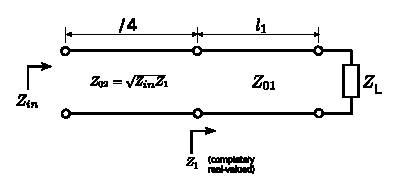
\includegraphics[width=\columnwidth]{modules/m0091_fQWM2.eps}
}}{A transmission line with three sets of parallel nodes extending from input and output branches. Starting at the top left and going clockwise, l equals lambda divided by 4 is measured between the source terminal and the middle terminal. l sub 1 is measured between the middle terminal and the load terminal. Z sub 01 is shown across the terminals on either side of the load. An arrow pointed toward the load originating at the middle terminal on the bottom side is labeled Z sub 1 (completely real-valued). }
\end{center} 
\caption{\label{m0091_fQWM2}Impedance-matching a complex-valued load impedance using quarter-wavelength transmission line.}
\end{figure}

%%%%%%%%%%%%%%%%%%%%%%%%%%%%%%%%%%%%%%%%%%%%%%%%%%%%%

%ORB EXAMPLE
~\\ \begin{example} 
\begin{mdframed}[backgroundcolor=brown!20,linecolor=brown!20]\raggedright
Matching a patch antenna 
\index{antenna!patch}
\index{patch antenna|see{antenna}}
\index{antenna!impedance matching}
to $50~\Omega$.
\\~\\
A particular patch antenna exhibits a source impedance of $Z_A = 35+j35~\Omega$. 
(See ``Microstrip antenna'' in ``Additional Reading'' at the end of this section for some optional reading on patch antennas.) 
Interface this antenna to $50~\Omega$ using the technique described above.
For the section of transmission line adjacent to the patch antenna, use characteristic impedance $Z_{01}=50~\Omega$.
Determine the lengths $l_1$ and $l_2$ of the two segments of transmission line, and the characteristic impedance $Z_{02}$ of the second (quarter-wave) segment. 

{\bf Solution.}
The length of the first section of the transmission line (adjacent to the antenna) is determined using Equation~\ref{m0093_eZ}:
%
\begin{equation}
Z_1(l_1) = Z_{01} \frac{ 1 + \Gamma e^{-j2\beta_1 l_1} }{  1 - \Gamma e^{-j2\beta_1 l_1} }
\end{equation}
%
where $\beta_1$ is the phase propagation constant for this section of transmission line and 
%
\begin{equation}
\Gamma \triangleq \frac{Z_A-Z_{01}}{Z_A+Z_{01}} \cong -0.0059+j0.4142
\end{equation}
%
We seek the value of smallest positive value of $\beta_1 l_1$ for which the imaginary part of $Z_1(l_1)$ is zero.
This can determined using a Smith chart  (see ``Additional Reading'' at the end of this section) or simply by a few iterations of trial-and-error.
Either way we find $Z_1(\beta_1 l_1 = 0.793~\mbox{rad}) \cong 120.719-j0.111~\Omega$, which we deem to be close enough to be acceptable.
Note that $\beta_1 = 2\pi/\lambda$, where $\lambda$ is the wavelength of the signal in the transmission line.
Therefore 
%
\begin{equation}
l_1 
= \frac{\beta_1 l_1}{\beta_1} 
= \frac{\beta_1 l_1}{2\pi} \lambda 
\cong 0.126\lambda
\end{equation} 

The length of the second section of the transmission line, being a quarter-wavelength transformer, should be $l_2 = 0.25\lambda$.
Using Equation~\ref{m0091_eQWZ0}, the characteristic impedance $Z_{02}$ of this section of line should be
%
\begin{equation}
Z_{02} \cong \sqrt{\left(120.719~\Omega\right) \left(50~\Omega\right) } \cong 77.7~\Omega
\end{equation}

%By the way, patch antennas often appear in systems implemented on printed circuit boards, 
%\index{printed circuit board (PCB)}
%because they themselves are easily implemented on printed circuit boards. 
%A great follow-up to this example would be to complete the solution in microstrip (Section~\ref{m0082_Microstrip_Line}) by determining the width of lines given a particular substrate and dielectric thickness.

{\bf Discussion.}
The total length of the matching structure is $l_1+l_2 \cong 0.376\lambda$.
A patch antenna would typically have sides of length about $\lambda/2 = 0.5\lambda$, so the matching structure is nearly as big as the antenna itself.
At frequencies where patch antennas are commonly used, and especially at frequencies in the UHF (300--3000~MHz) band, patch antennas are often comparable to the size of the system, so it is not attractive to have the matching structure also require a similar amount of space.
Thus, we would be motivated to find a smaller matching structure.

\end{mdframed}\end{example}

%%%%%%%%%%%%%%%%%%%%%%%%%%%%%%%%%%%%%%%%%%%%%%%%%%%%

Although quarter-wave matching techniques are generally effective and commonly used, they have one important contraindication, noted above --  They often result in structures that are large. That is, any structure which employs a quarter-wave match will be at least $\lambda/4$ long, and $\lambda/4$ is typically large compared to the associated electronics.  
Other transmission line matching techniques -- and in particular, single stub matching (Section~\ref{m0094_Single-Stub_Matching}) -- typically result in structures which are significantly smaller. 

The impedance inversion property of quarter-wavelength lines has applications beyond impedance matching.  
The following example demonstrates one such application:

%ORB EXAMPLE
~\\ \begin{example} 
\begin{mdframed}[backgroundcolor=brown!20,linecolor=brown!20]\raggedright
RF/DC decoupling in transistor amplifiers.
\index{amplifier}
\\~\\
Transistor amplifiers for RF applications often receive DC current at the same terminal which delivers the amplified RF signal, as shown in Figure~\ref{m0091_BiasT}.
The power supply typically has a low output impedance.
If the power supply is directly connected to the transistor, then the RF will flow predominantly in the direction of the power supply as opposed to following the desired path, which exhibits a higher impedance.
This can be addressed using an inductor in series with the power supply output.
This works because the inductor exhibits low impedance at DC and high impedance at RF.
Unfortunately, discrete inductors are often not practical at high RF frequencies.
This is because practical inductors also exhibit parallel capacitance, which tends to \emph{decrease} impedance.  

A solution is to replace the inductor with a transmission line having length $\lambda/4$ as shown in Figure~\ref{m0091_QWDecoupling}.
A wavelength at DC is infinite, so the transmission line is essentially transparent to the power supply.
At radio frequencies, the line transforms the low impedance of the power supply to an impedance that is very large relative to the impedance of the desired RF path.
Furthermore, transmission lines on printed circuit boards are much cheaper than discrete inductors (and are always in stock!).

\end{mdframed}
%
\begin{figure}
\begin{center}
\pdftooltip{{  % note double braces
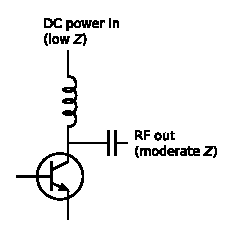
\includegraphics[width=1.5in]{modules/m0091_fBiasT.eps}
}}{A common-emitter RF amplifier in series with an inductor and a capacitor. Starting at the top, the words “DC power in (low Z)” are written above the inductor symbol. Connected at a perpendicular angle is a capacitor, with the words “ RF out (moderate Z)” written directly to the right. Intersection of inductor and capacitor connected to common branch of common-emitter RF amplifier. }
\end{center} 
\caption{\label{m0091_BiasT}Use of an inductor to decouple the DC input power from the RF output signal at the output of a common-emitter RF amplifier.}
\end{figure}
%
\begin{figure}
\begin{center}
\pdftooltip{{  % note double braces
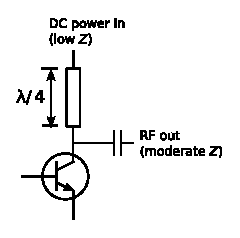
\includegraphics[width=1.5in]{modules/m0091_fQWDecoupling.eps}
}}{Similar layout to a previous figure.  A quarter wavelength transmission line shown as a rectangle. “DC power in (low Z)” is written above the transmission line symbol. Capacitor connected perpendicular “ RF out (moderate Z)” written directly to the right. Shared transmission line-capacitor node connected to common of a common-emitter RF amplifier. }
\end{center} 
\caption{\label{m0091_QWDecoupling}Decoupling of DC input power and RF output signal at the output of a common-emitter RF amplifier, using a quarter-wavelength transmission line.}
\end{figure}
%
\end{example}

%%% TODO Problem ECE3106 17Sp MP2 problem that does the above


{\bf Additional Reading:}
\begin{itemize}
\item ``\href{https://en.wikipedia.org/wiki/Quarter-wave_impedance_transformer}{\small Quarter-wavelength impedance transformer}'' on Wikipedia.
\item ``\href{https://en.wikipedia.org/wiki/Smith_chart}{\small Smith chart}'' on Wikipedia.
\item ``\href{https://en.wikipedia.org/wiki/Microstrip_antenna}{Microstrip antenna}'' on Wikipedia.
\end{itemize}

\index{transmission line!quarter-wavelength|)}
